\chapter[Embasamento Teórico]{Embasamento Teórico}

\section{Engenharia de Requisitos} 

Por se tratar de uma área que se encontra entre o abstrato e o concreto, Westfall \cite{westfall_5w2h}, em seu estudo, busca definir os diferentes porquês da existência da Engenharia de Requisitos, sendo:

\begin{itemize}
    \item O que é?: são os requerimentos responsáveis pela definição do que o \textit{software} deve fazer (\textit{requisito funcional}\footnote{Declarações de serviços que o sistema deve prover, como deve reagir para entradas e como deve se comportar em situações especificas \cite{sommerville2011}.}) e possuir (\textit{requisitos não funcionais}\footnote{Restrições aos serviços ou funções oferecidas pelo sistema. Aplicam-se ao sistema como um todo \cite{sommerville2011}.}) para agregar valor para os seus \textit{stakeholders}\footnote{Grupo de pessoas interessadas no produto, podendo ser cliente, usuários etc.}; Existem vários níveis e tipos diferentes de requisitos, que são mostrados na Figura \ref{lev_tipo_req}:
    
    \begin{figure}[htb]
        \begin{center}
            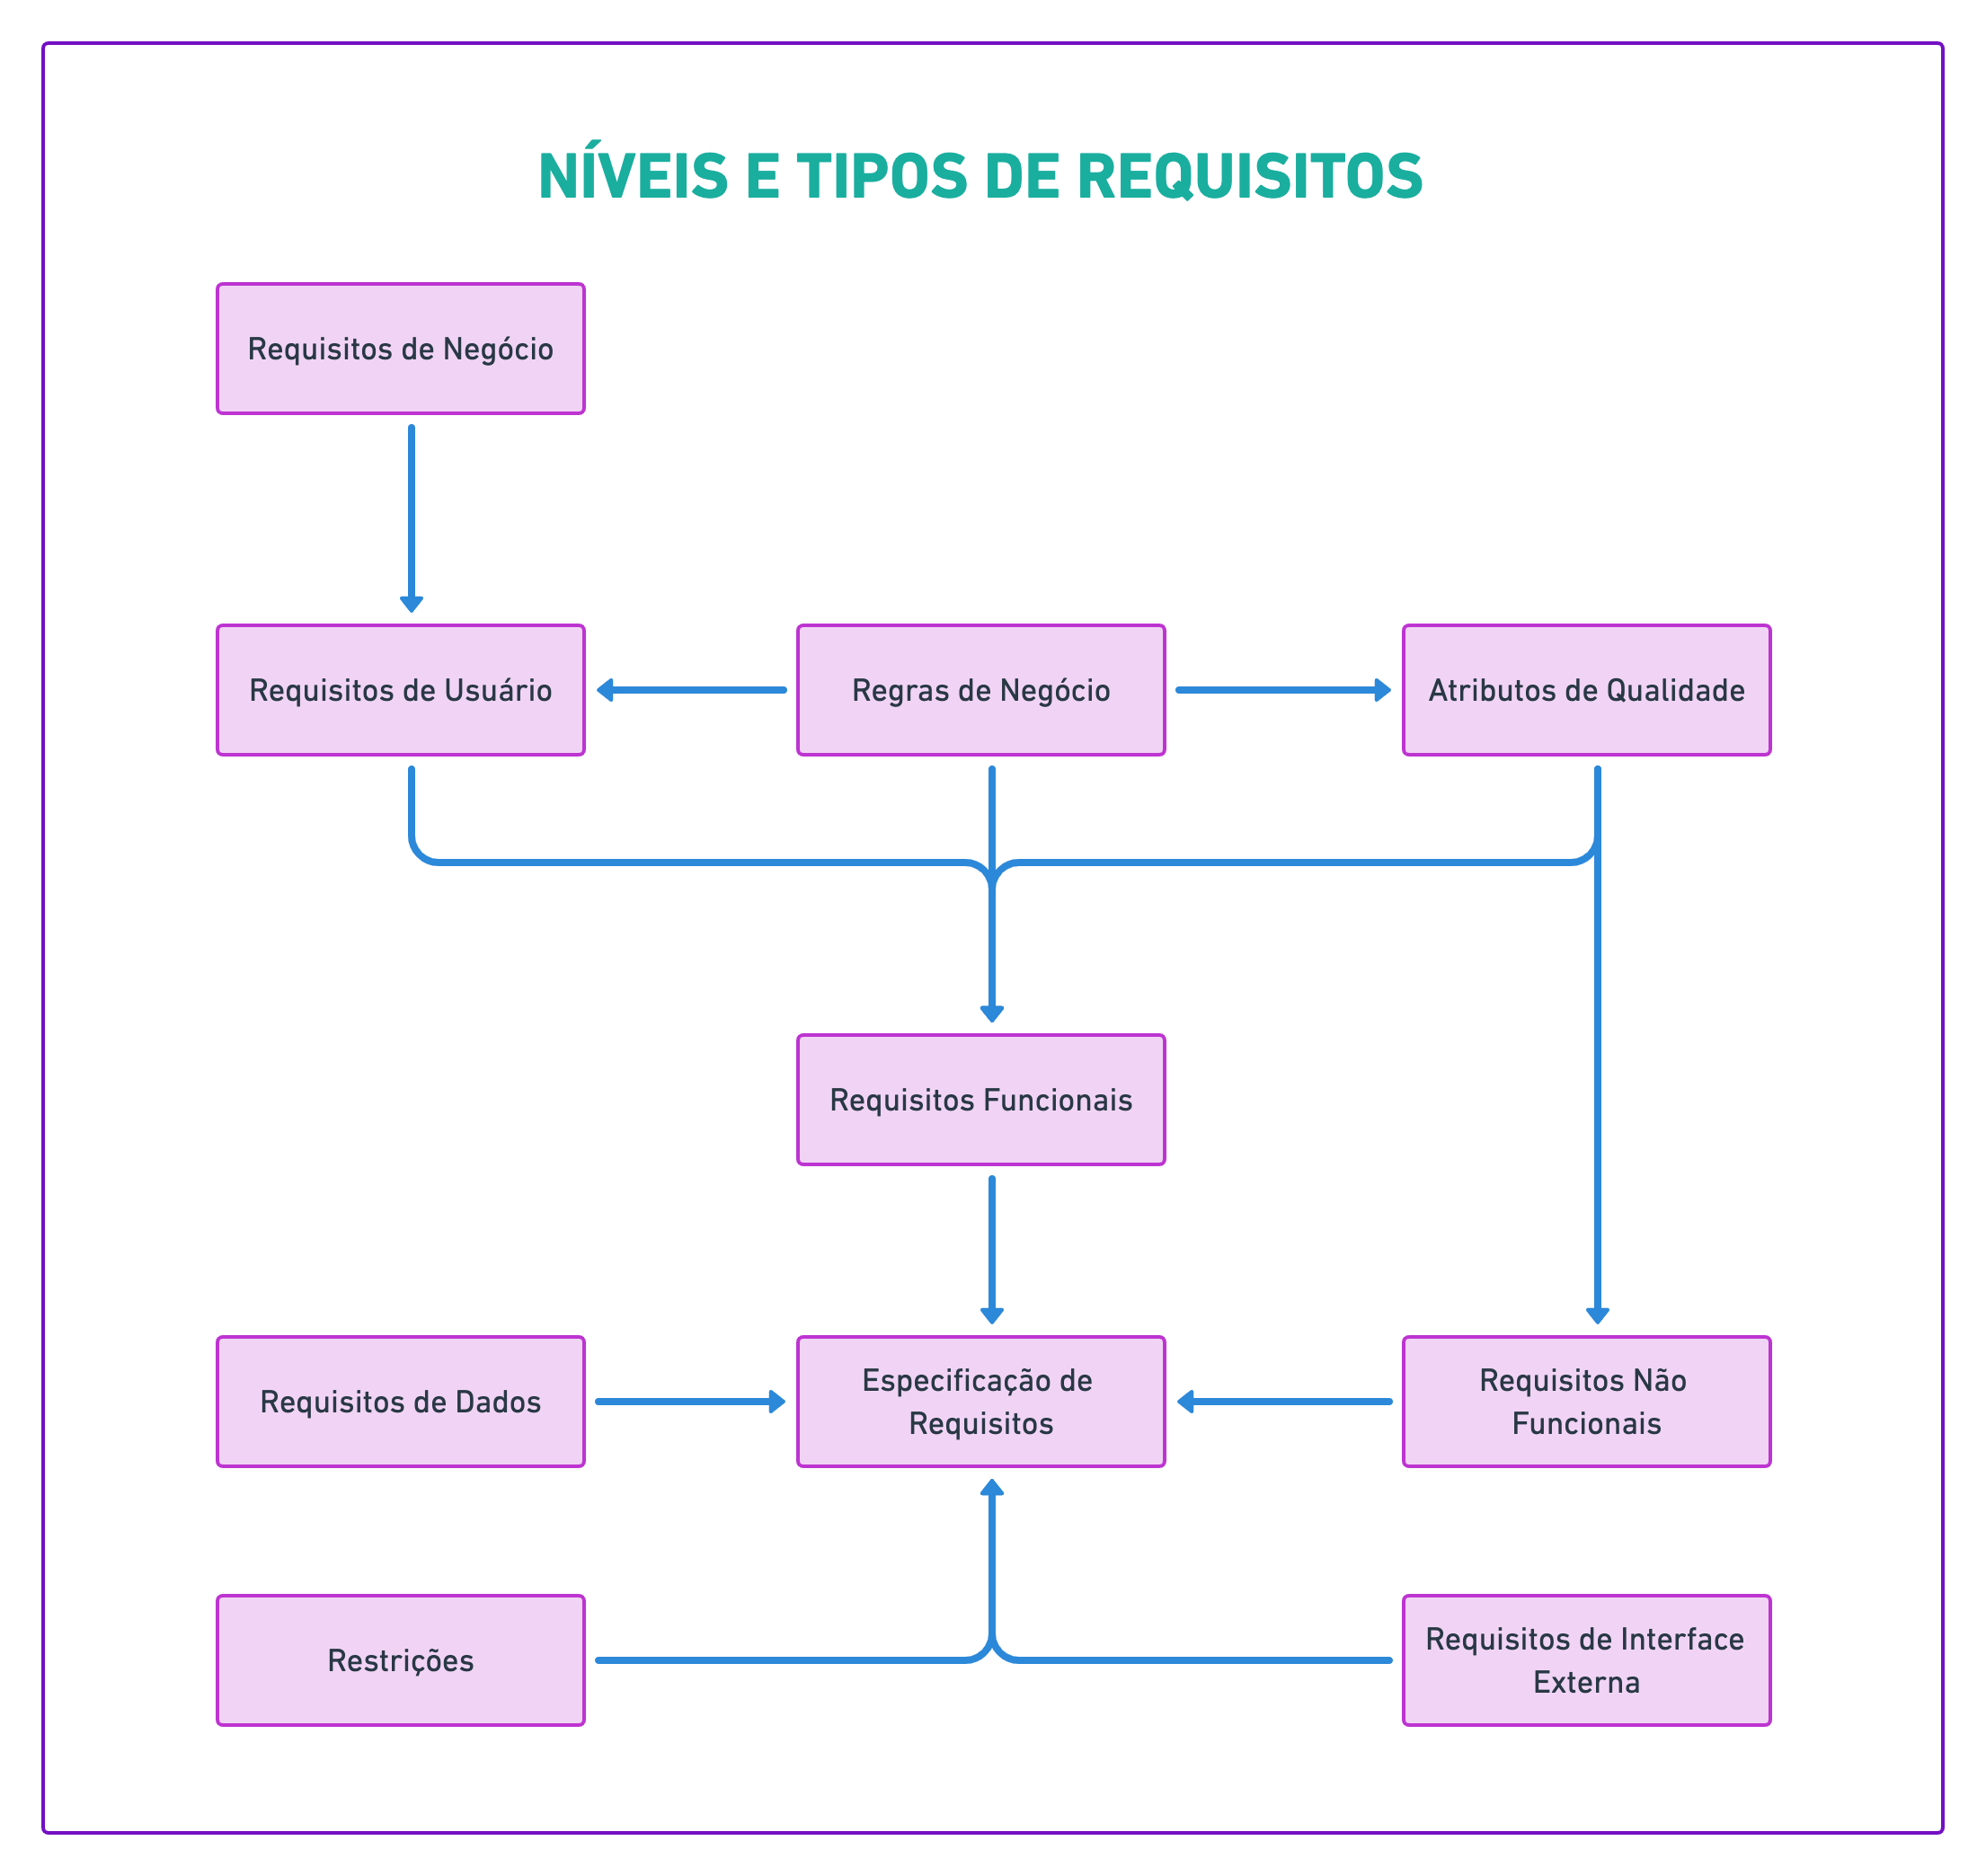
\includegraphics[width=12cm, height=10cm, keepaspectratio]{figuras/lev_tipo_req.png}
            \caption{{Níveis e Tipos de Requisitos. \cite{westfall_5w2h}}}
            \label{lev_tipo_req}
        \end{center}
    \end{figure}
    
    \begin{itemize}
    
        \item Os \textbf{requisitos de negócio} definem, de forma direta, quais são os problemas que devem ser resolvidos e por que o produto de \textit{software} está sendo desenvolvido;
        
        \item Os \textbf{requisitos de usuário} têm o objetivo de visualizar as funcionalidades do produto de \textit{software} a partir da perspectiva do usuário. De forma resumida, eles definem o que o \textit{software} deve realizar para que os usuários atinjam seus objetivos;
        
        \item Os \textbf{requisitos funcionais} de produto definem as funcionalidades do software que devem ser implementadas para que os usuários consigam realizar suas tarefas de forma fácil;
        
        \item As regras de negócio são declarações sobre a forma da empresa fazer negócio, ou seja, elas refletem as políticas, os padrões, as práticas, os regulamentos e as diretrizes de negócio;
        
        \item Os \textbf{atributos de qualidade} no nível de usuário definem requisitos não funcionais que determinam o produto de \textit{software}. Incluem confiabilidade, disponibilidade, segurança, manutenibilidade, portabilidade, usabilidade, dentre outros;
        
        \item Os requisitos\textbf{ de interface externa}, de forma objetiva, definem o fluxo de informações através de interfaces compartilhadas;
        
        \item As \textbf{restrições} têm o objetivo de mostrar quais destas limitações foram colocadas pelo fornecedor ao projetar e desenvolver o \textit{software} e
        
        \item Os requisitos de dados definem os itens de dados específicos que devem ser introduzidos como parte do produto de \textit{software}.
    
    \end{itemize}
    
    \item Para que serve? : um dos grandes nomes da engenharia de \texit{software}, Fred Brooks, afirma que
        \begin{citacao}
        A parte mais difícil da construção de um sistema de \textit{software} é decidir precisamente o que deve ser feito. Nenhuma outra parte do trabalho conceitual é tão  custoso quanto estabelecer detalhadamente os requisitos técnicos, incluindo todas as interfaces para os usuários, para os computadores, e para os outros sistemas do \textit{software}. Nenhuma outra parte do trabalho prejudica tanto o sistema se for feita de maneira errada. Nenhuma outra parte é tão difícil de ser retificada posteriormente \cite[p.~199]{brooks1995mythical}.
        \end{citacao}
    Assim, pode-se entender o quão crítico é esse fase do processo de desenvolvimento de \texit{software}, contexto que se insere esse trabalho;
    
    \item Para quem?: os \textit{stakeholders} são indivíduos que impactam ou que são impactados pelo produto de \textit{software} e, portanto, possuem um nível de influência sobre o produto. Dentro desse contexto, existem diferentes perspectivas relacionadas à atuação de cada indivíduo, sendo os mais comuns:
    
    \begin{itemize}
        \item Os Analistas de Requisitos são essenciais dentro dessa área pelo fato deles serem responsáveis pela elicitação, análise e especificação dos requisitos, além de comunicar os requisitos aos desenvolvedores e às partes interessadas;
    
        \item Os Arquitetos de \textit{Software} são essenciais por criarem toda a arquitetura do \textit{software} a partir dos requisitos elicitados e por dizerem como vai ser implementado;
    
        \item Já os desenvolvedores são responsáveis pela implementação o produto de \textit{software}, traduzindo os requisitos em funcionalidades concretas;
    
        \item Os Testadores de \textit{Software} têm o objetivo de usar os requisitos elicitados como base, e criar casos de teste para que o produto de \textit{software} seja testado sob condições específicas, afim de detectar defeitos para que, após os testes, passem confiabilidade de que o produto de \textit{software} esteja funcionando de acordo com as características estabelecidas;
    
        \item Os Gerentes de Projeto são responsáveis pelo planejamento e pelo monitoramento de todos os envolvidos no projeto, além de guiar o time de desenvolvimento de \textit{software} para que o produto final seja entregue com todos os requisitos definidos anteriormente e,
    
        \item O Gerente do Produto é uma peça fundamental dentro desse processo, pois revisa todas as mudanças propostas; analisa os riscos e os impactos que podem vir a ocorrer, e aprova ou desaprova quaisquer mudanças, garantindo que essas mudanças foram implementadas e validadas.
    \end{itemize}
    
    \item Quando?: a maior parte do processo da Engenharia de Requisitos é feita nas primeiras fases do ciclo de vida do produto, contudo não deve ser restrito somente a esse período, uma vez que novos requisitos vão surgindo e o projeto deve se adaptar às novas realidades, pois deve ser um processo iterativo. Esse aspecto está ligado ao gerenciamento de requisitos, o qual necessita avaliar como novas requisições influenciam no desenvolvimento do projeto, assim como elencar os riscos e impactos causados por essas alterações. Posteriormente, após a aprovação, ocorre a implementação da nova funcionalidade. Durante a fase de desenvolvimento, estes requisitos devem ser usados como critérios para testar o produto e validar a correta implementação das funcionalidades. Os requisitos de negócio devem ser os primeiros a serem modelados, seguidos dos requerimentos de usuário e, por fim, os de produto, e
    
    \item Como?: A Engenharia de Requisitos de \textit{software} é um processo bem definido, com etapas claras e repletas de documentações que possam registrar e orientar o desenvolvimento do produto. O desenvolvimento e a gerência dos requisitos são dois grandes processos dentro deste escopo. A Figura \ref{eng_req_flux} representa bem essas etapas e subetapas do processo da Engenharia de Requisitos que vão ser mais bem especificadas no decorrer deste trabalho.
    
    \begin{figure}[htb]
        \begin{center}
            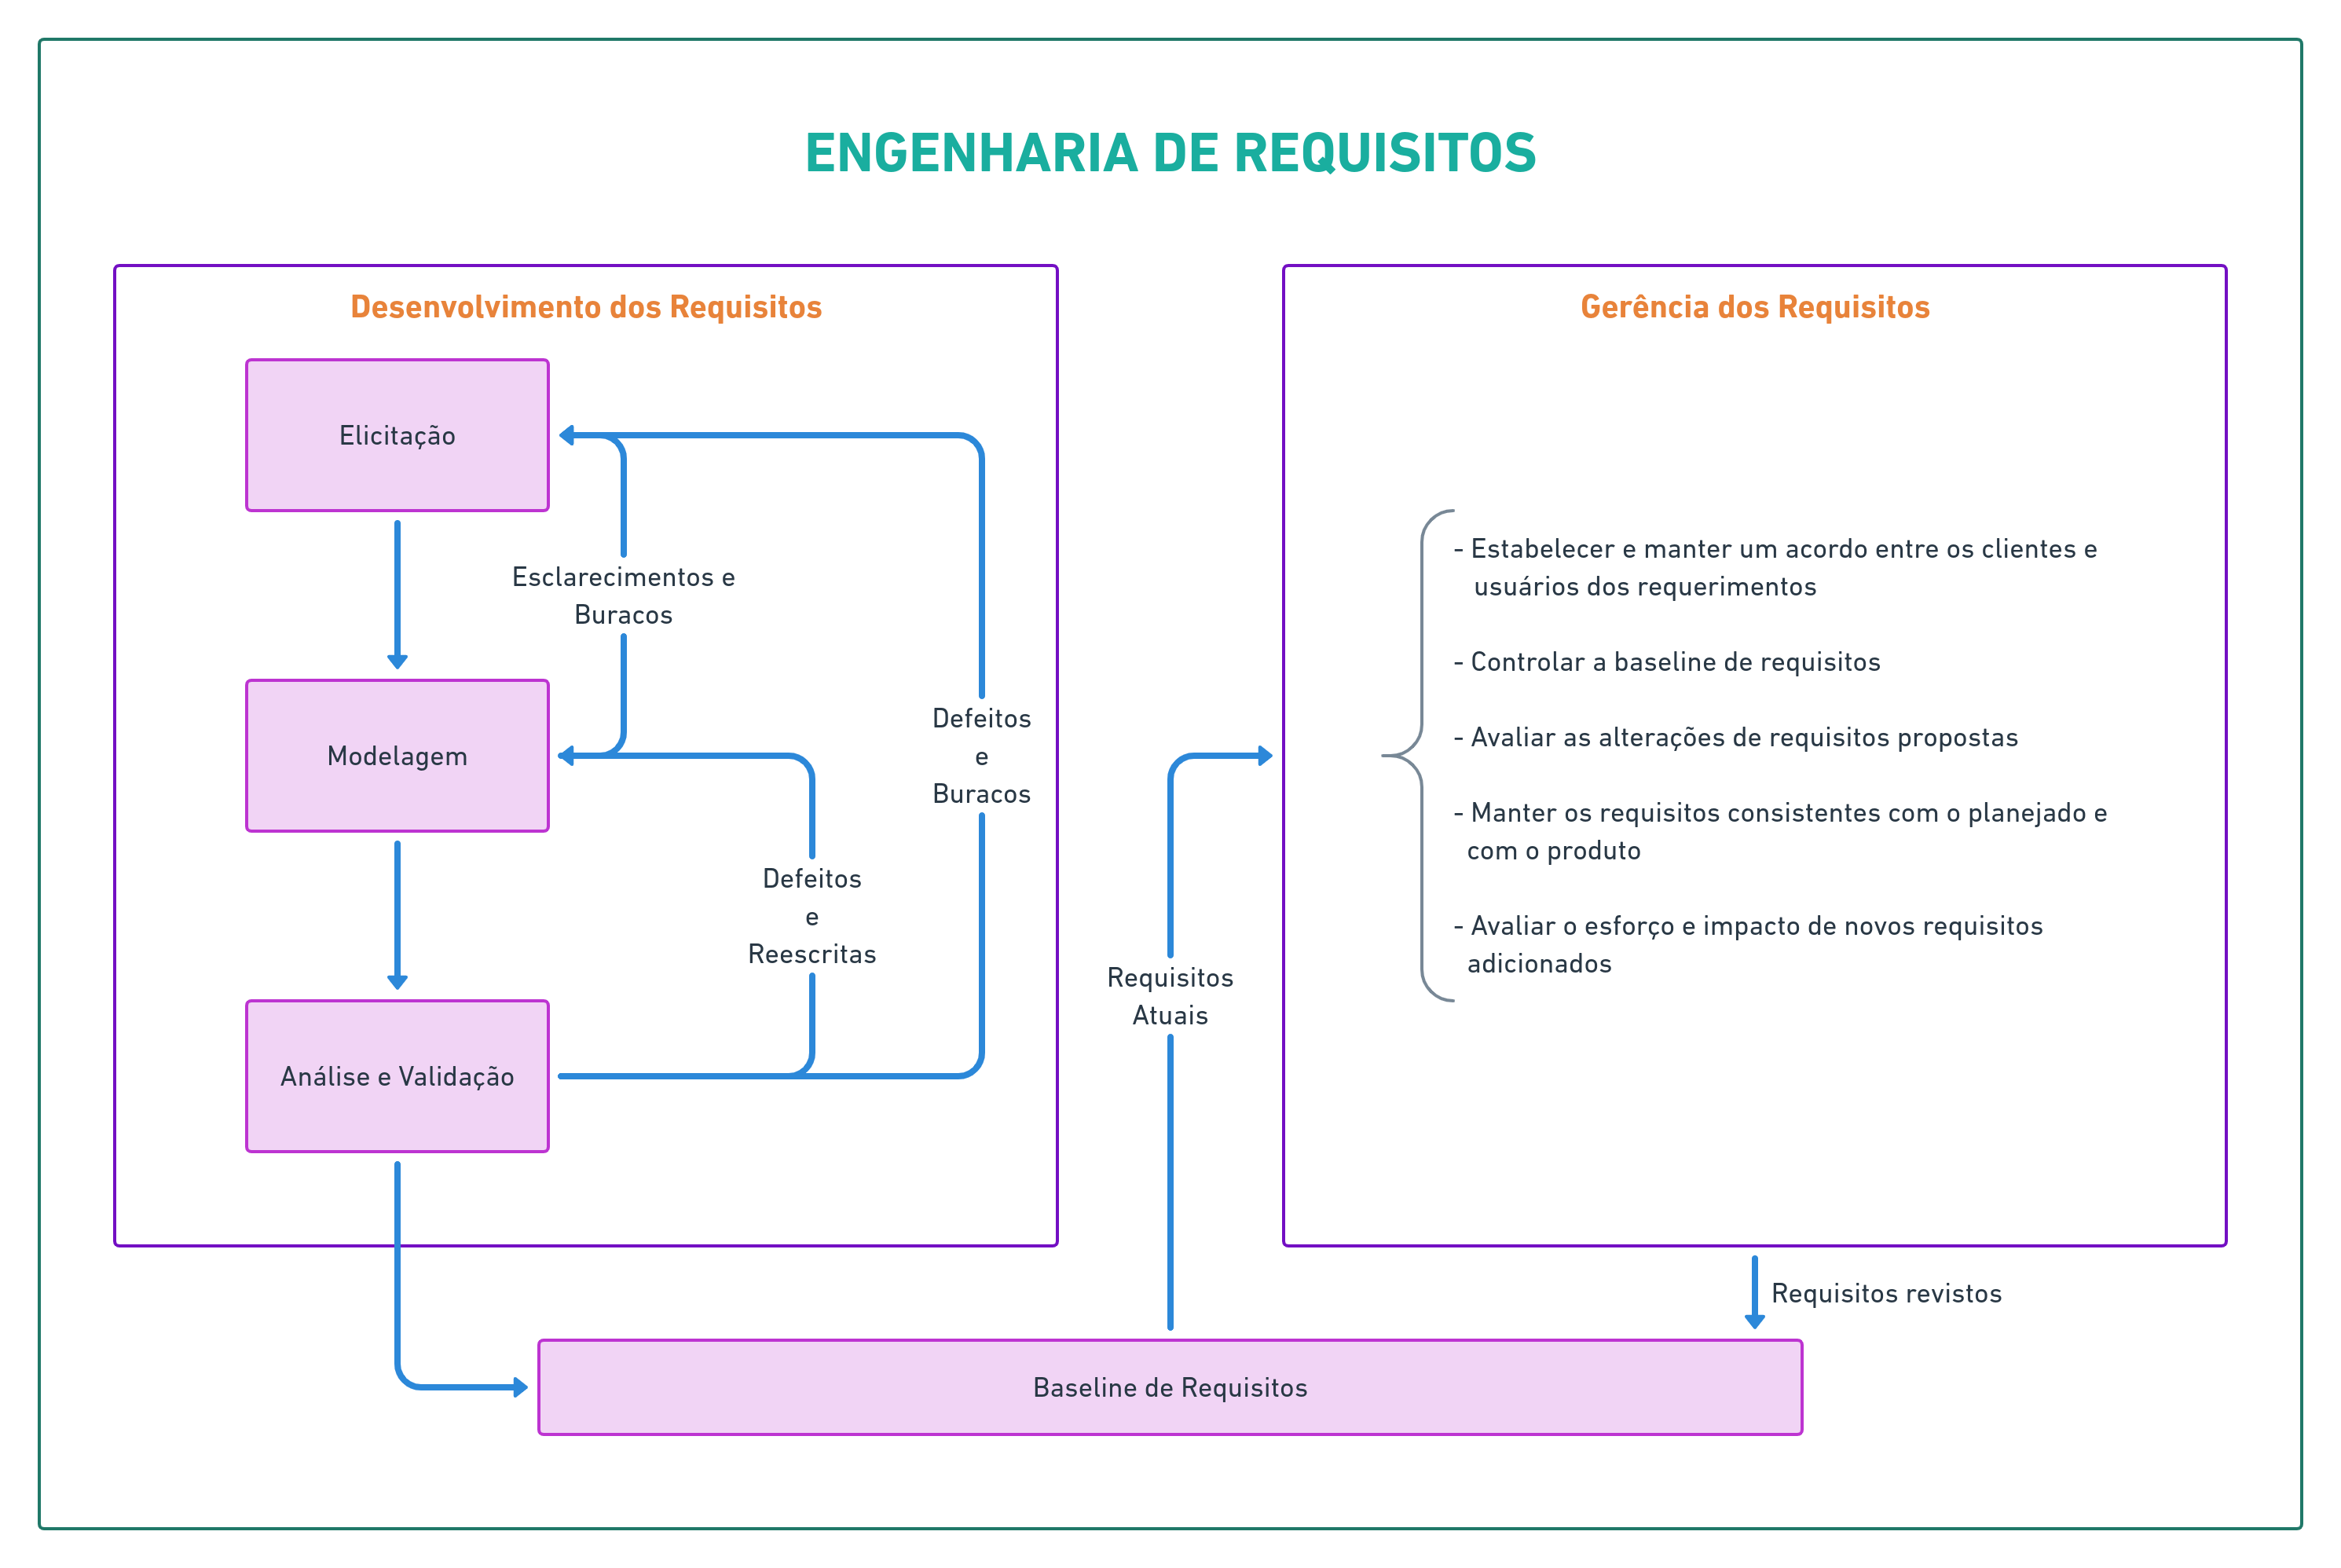
\includegraphics[width=12cm,height=12cm,keepaspectratio]{figuras/Introducao/eng_req_fluxo.png}
            \caption{{Fluxo da Engenharia de Requisitos. Adaptado de \cite{westfall_5w2h}}}
            \label{eng_req_flux}
        \end{center}
    \end{figure}
    
\end{itemize}

Como vimos, a Engenharia de Requisitos é uma área essencial dentro da construção de um produto de \textit{software}. Existem vários processos e várias técnicas utilizadas para que o produto final seja desenvolvido com qualidade, evitando problemas no futuro.

Algum dos processos e técnicas utilizadas dentro da Engenharia de Requisitos serão faladas a seguir.

\subsubsection{Rich Picture}

\subsubsection{5W2H}

\subsection {Elicitação}
A Elicitação de Requisitos é o processo relacionado com as atividades que permitem a compreensão de metas, objetivos e motivos para a construção de um novo sistema de \textit{software} e a identificação de todos os requisitos das partes interessadas que facilitarão o sistema a ser desenvolvido \cite{elliott2012software}. Além disso, as informações coletadas durante a elicitação de requisitos geralmente precisam ser interpretadas, analisadas, modeladas e validadas antes do início da implementação do sistema \cite{nuseibeh2000requirements}.

\subsubsection{Brainstorming}

\subsubsection{Questionário}

\subsubsection{Protótipo de Baixa Fidelidade}

\subsubsection{Storytelling}

\subsubsection{Entrevista}

\subsubsection{Análise de Protocolo}

\subsection {Modelagem}

\subsubsection{Backlog}

\subsubsection{NFR}

\subsubsection{Léxicos}

\subsection {Verificação}

\subsection {Pós-rastreabilidade}

\subsubsection{Priorização (MVP)}

\subsubsection{Backward-from}

\subsection {Rastreabilidade}
A rastreabilidade é um tópico essencial dentro da Engenharia de Requisitos, pois é utilizado para providenciar relações entre requisitos, arquitetura e implementação final do sistema, além de possibilitar uma compreensão dos relacionamentos de dependência entre os requisitos propostos. Dessa forma, a rastreabilidade pode ser implementada como um conjunto de ligações entre os requisitos \cite{sayao2006rastreabilidade}.

A rastreabilidade tem o objetivo de acompanhar e descrever o ciclo de um requisito de duas formas:
\begin{itemize}
    \item Pré-rastreabilidade: documentar o contexto a partir do qual emergem os requisitos;
    \item Pós-rastreabilidade: vincula os requisitos à arquitetura do sistema e sua implementação.
\end{itemize}